\chapter{Five Online Businesses and the Discipline of Choosing}

This chapter follows a School of Hard Knocks entrepreneurship interview curated by LazyingArt LLC through Video2Book. The lecture is not a blackboard derivation; it is a practical classification of five online business models. We will read it in that spirit: each model has an asset to build, a buyer or audience, a channel, and a bottleneck that makes the work harder than it first appears.

\section{Choosing by Endurance, Not Hype}

The speaker begins by lowering the temperature. He is not there to sell a course or push a product. He is offering his own view of five online businesses worth considering in 2022. That opening matters because the list is not meant to function as a promise. It is a menu of possible work.

Before the first business appears, the real selection rule is already on the table. We should not ask only which business is popular. We should ask which one we can keep doing long enough to become good at it.

\begin{equation}
N_{\mathrm{models}} = 5 .
\end{equation}

The five models are

\begin{equation}
\mathcal{B}
=
\{\text{creator work},\ \text{video editing},\ \text{e-commerce},\ \text{social media marketing},\ \text{online courses}\}.
\end{equation}

The lecture's first practical equation is therefore not a revenue equation. It is a fit equation:

\begin{equation}
\mathrm{fit}
\approx
\mathrm{interest}
+
\mathrm{capacity\ for\ repeated\ work}.
\end{equation}

This is only a compact notation for the speaker's point, not a literal formula. But it captures the governing idea. The business that looks impressive from the outside may fail if the daily work is intolerable. The business that keeps one's attention has a better chance of surviving the long middle period where skill is being built and results are still uneven.

\begin{figure}
\centering
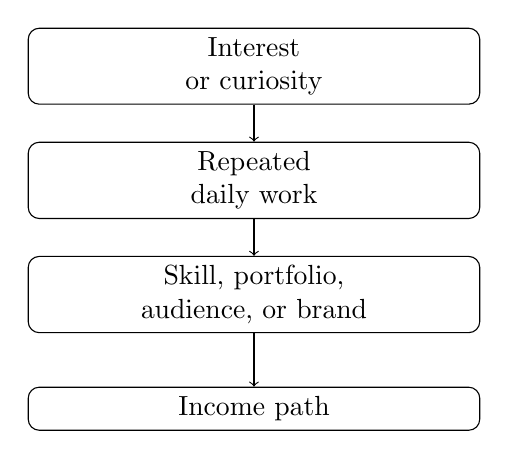
\begin{tikzpicture}[x=1cm,y=1cm]
\node[draw, rounded corners, align=center, text width=5.5cm] (interest) at (0,0) {Interest\\or curiosity};
\node[draw, rounded corners, align=center, text width=5.5cm] (work) at (0,-1.45) {Repeated\\daily work};
\node[draw, rounded corners, align=center, text width=5.5cm] (asset) at (0,-2.9) {Skill, portfolio,\\audience, or brand};
\node[draw, rounded corners, align=center, text width=5.5cm] (income) at (0,-4.35) {Income path};
\draw[->] (interest) -- (work);
\draw[->] (work) -- (asset);
\draw[->] (asset) -- (income);
\end{tikzpicture}
\caption{The opening filter: interest is valuable because it helps sustain the repetition needed to build a useful asset.}
\end{figure}

\section{Creator Work: Audience as an Asset}

At number one, the speaker names creator work. He immediately splits it into two routes. The first is to build a personal brand around oneself: vlogs, gaming, business content, or any other content identity. The second is to create content for an existing brand.

\begin{equation}
\mathrm{creator\ work}
=
\mathrm{personal\ brand}
\quad \hbox{or} \quad
\mathrm{content\ for\ brands}.
\end{equation}

The personal-brand route is attractive because one audience can support several income paths. The speaker names ad revenue from platforms such as TikTok and YouTube, brand deals, and later businesses built from audience trust. A creator who has earned attention can sometimes extend that attention into products such as skincare, clothing, or another line connected to the creator's name.

The brand-deal figure is given as an example range:

\begin{equation}
D_{\mathrm{deal}}
\approx
\$500 \hbox{ to } \$5{,}000
\quad \hbox{per promotion}.
\end{equation}

The mechanism is the main point:

\begin{align}
\mathrm{personal\ brand}
&\longrightarrow
\mathrm{audience},\\
\mathrm{audience}
&\longrightarrow
\{\mathrm{ad\ revenue},\ \mathrm{brand\ deals},\ \mathrm{new\ businesses}\}.
\end{align}

The second creator route is more immediately service-like. Companies need content daily: user-generated content, reviews, product explanations, and event announcements. The speaker mentions JT Barnett as an example of someone working around the problem of connecting creators with companies so that creators can become the face of new brands.

\subsection{Question \& Answer}

\paragraph{Question.}
What if we want to build a personal brand, but our own brand cannot yet support us full time?

\paragraph{Answer.}
The lecture's answer is to separate the long-term asset from the near-term service. We can build the personal brand in the background while selling content creation to other brands in the foreground.

\begin{align}
\mathrm{early\ creator}
&=
\mathrm{personal\ brand\ under\ construction}
+
\mathrm{brand\ content\ services},\\
\mathrm{brand\ content\ services}
&\longrightarrow
\mathrm{cash\ flow\ while\ the\ audience\ grows}.
\end{align}

That is the first real commercial bridge in the lecture. Owned audience may be the long-term asset, but service work can make the craft economically possible before the audience is large enough.

\section{Video Editing: Selling Time Back to Creators}

At number two, the lecture moves behind the camera. Video editing is for someone who likes the content creation space but does not want to be in front of the camera all the time. The speaker adds a useful qualification: an editor should have an eye for what makes content good or enjoyable, which usually means studying and consuming content regularly.

The demand argument is not mysterious. It is a time-allocation problem. Companies are moving more heavily into digital channels, and creators often do not have time to break one piece of content into all the formats the platforms demand. A YouTube vlogger may need short clips for TikTok, Instagram, and a YouTube clips channel. That work has to be done by someone.

Let \(T_{\mathrm{repurpose}}\) denote the time needed to cut and adapt content across platforms. Let \(T_{\mathrm{creator}}\) denote the time the creator can afford to spend on that task. The opportunity appears when

\begin{equation}
T_{\mathrm{repurpose}} > T_{\mathrm{creator}} .
\end{equation}

The editor sells the difference:

\begin{equation}
\mathrm{editor\ value}
\approx
\mathrm{saved\ time}
+
\mathrm{platform-ready\ output}.
\end{equation}

\paragraph{A worked entry path.}
The speaker's entry path is simple and practical.

\begin{enumerate}
\item Learn the craft from online resources such as YouTube, Google, Udemy, and Skillshare.
\item Study strong working editors; the speaker names Hillier Smith, associated with editing for Logan Paul.
\item Offer services on platforms such as Fiverr and Upwork.
\item Use early jobs to build proof before approaching larger creators or brands.
\end{enumerate}

As a small update rule, portfolio-building looks like

\begin{equation}
P_{n+1}
=
P_n
+
W_n ,
\end{equation}

where \(P_n\) is the portfolio after \(n\) completed jobs and \(W_n\) is the next piece of completed client work. The point is not that marketplaces are the whole career. The point is that they can produce visible evidence that the editor can deliver.

\section{E-Commerce: Scale With Operational Demands}

At number three, the lecture turns from media service to product ownership. E-commerce is attractive when someone makes a product, wants to sell a particular item, or wants to build an online clothing brand. The upside is scale. A product brand can become larger than the founder, and in the speaker's optimistic framing it can even become something that lasts beyond one generation.

Then the tone changes. The speaker immediately adds that e-commerce is one of the harder business models to start. It requires business judgment, marketing skill, and the ability to acquire customers consistently.

The warning can be compressed as

\begin{equation}
\mathrm{sustainable\ e\mbox{-}commerce}
\neq
\mathrm{launch\ customers\ only}.
\end{equation}

A launch can create the first burst of demand, but it does not solve the next eleven months. The business has to keep finding customers:

\begin{equation}
C_{\mathrm{year}}
=
C_{\mathrm{launch}}
+
\sum_{m=2}^{12} C_m ,
\end{equation}

where \(C_m\) denotes customers acquired in month \(m\). This notation is our reconstruction of the business logic, but the underlying claim is directly from the lecture: getting customers at launch is not the same as getting customers all year.

There is also a capital constraint. The speaker names two uses of startup money: product and marketing.

\begin{equation}
K_{\mathrm{startup}}
=
K_{\mathrm{product}}
+
K_{\mathrm{marketing}}.
\end{equation}

The recommendation is not to avoid e-commerce. It is to enter it with the right expectations. If someone is passionate about clothing or a brand idea, the speaker's method is research: study other stores and brands, model what works, and then do the work directly.

\section{Social Media Marketing: Local Businesses and Monthly Retainers}

At number four, the lecture returns to service work, now with a local-business client. The speaker's example is a restaurant. The restaurant may already have good food and good customer service, but it may not be showing its products online.

That gives the service its shape:

\begin{equation}
\mathrm{good\ product/service}
+
\mathrm{weak\ online\ visibility}
\longrightarrow
\mathrm{marketing\ opportunity}.
\end{equation}

The proposed offer is monthly management. The marketer approaches the owner, identifies the online visibility gap, agrees on a fee, and then manages social media on a monthly basis. The example range is

\begin{equation}
R_{\mathrm{monthly}}
\approx
\$500 \hbox{ to } \$1{,}500
\quad \hbox{per month}.
\end{equation}

The baseline work is concrete: take pictures of the food and menu, learn about upcoming events, and post about them. But the lecture does not stop at posting. To separate oneself from weaker operators, the speaker recommends learning Facebook ads, Instagram ads, and other platform advertising systems.

\subsection{Question \& Answer}

\paragraph{Question.}
If the restaurant already has good food, good service, and real products, what problem are we solving?

\paragraph{Answer.}
We are solving visibility and reach, not the product itself. If the business starts with little or no following, posting can produce zero engagement and zero views. In that case, the owner spends money without receiving a return.

A compact decision rule is

\begin{equation}
\mathrm{organic\ reach} \approx 0
\quad \Longrightarrow \quad
\mathrm{posting\ alone\ is\ insufficient}.
\end{equation}

So the stronger offer is not merely ``we will post for you.'' It is closer to

\begin{align}
\mathrm{monthly\ management}
&=
\mathrm{content}
+
\mathrm{posting}
+
\mathrm{platform\ knowledge},\\
\mathrm{stronger\ offer}
&=
\mathrm{monthly\ management}
+
\mathrm{advertising\ ability}.
\end{align}

\begin{figure}
\centering
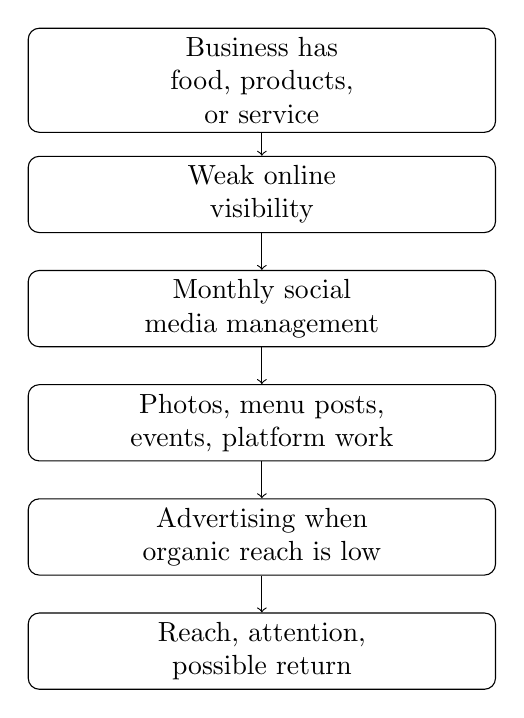
\begin{tikzpicture}[x=1cm,y=1cm]
\node[draw, rounded corners, align=center, text width=5.7cm] (product) at (0,0) {Business has\\food, products,\\or service};
\node[draw, rounded corners, align=center, text width=5.7cm] (visibility) at (0,-1.45) {Weak online\\visibility};
\node[draw, rounded corners, align=center, text width=5.7cm] (retainer) at (0,-2.9) {Monthly social\\media management};
\node[draw, rounded corners, align=center, text width=5.7cm] (content) at (0,-4.35) {Photos, menu posts,\\events, platform work};
\node[draw, rounded corners, align=center, text width=5.7cm] (ads) at (0,-5.8) {Advertising when\\organic reach is low};
\node[draw, rounded corners, align=center, text width=5.7cm] (return) at (0,-7.25) {Reach, attention,\\possible return};
\draw[->] (product) -- (visibility);
\draw[->] (visibility) -- (retainer);
\draw[->] (retainer) -- (content);
\draw[->] (content) -- (ads);
\draw[->] (ads) -- (return);
\end{tikzpicture}
\caption{The restaurant example: the service begins with visibility, but the deeper promise is reach and possible return.}
\end{figure}

\section{Online Courses: Packaging Expertise for Reach}

At number five, the lecture turns expertise into a product. An online course makes sense when someone is already skilled at something or successful in a field and can teach a process. The transcript is garbled in one phrase, but the surrounding meaning is clear: the course should give students an A-to-Z framework they can adapt in their own way.

The speaker's example is a custom shoe design business. A course could teach the materials, the starting steps, how to work on different shoes, and the practical process behind the business.

The structure is

\begin{align}
\mathrm{expertise}
&\longrightarrow
\mathrm{framework},\\
\mathrm{framework}
&\longrightarrow
\mathrm{course},\\
\mathrm{course}
&\longrightarrow
\mathrm{additional\ income\ stream}.
\end{align}

The speaker is careful not to oversell this model. He frames it more as a side hustle or additional income stream than as the central business. Distribution is the reason to use course platforms. Udemy and Skillshare can expose the course to buyers beyond existing followers and personal contacts.

\begin{equation}
\mathrm{course\ reach}
=
\mathrm{existing\ audience}
+
\mathrm{marketplace\ audience}.
\end{equation}

This is the same underlying pattern again: an asset becomes more valuable when paired with a channel. Expertise is private until it is packaged. A course packages it. A marketplace increases its surface area.

\section{The Five Models as a Working Map}

The lecture is a list, but under the list is a repeated structure. Each business asks us to build a different asset and face a different bottleneck. The following reconstruction is not a board diagram; it is a compact map of the lecture's commercial logic.

\begin{figure}
\centering
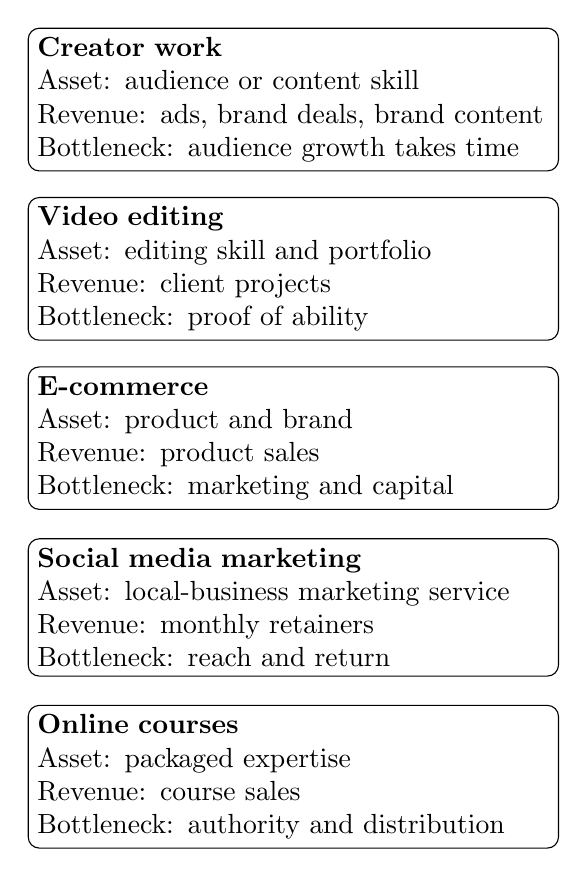
\begin{tikzpicture}[x=1cm,y=1cm]
\node[draw, rounded corners, align=left, text width=6.5cm] at (0,0)
{\textbf{Creator work}\\
Asset: audience or content skill\\
Revenue: ads, brand deals, brand content\\
Bottleneck: audience growth takes time};

\node[draw, rounded corners, align=left, text width=6.5cm] at (0,-2.15)
{\textbf{Video editing}\\
Asset: editing skill and portfolio\\
Revenue: client projects\\
Bottleneck: proof of ability};

\node[draw, rounded corners, align=left, text width=6.5cm] at (0,-4.3)
{\textbf{E-commerce}\\
Asset: product and brand\\
Revenue: product sales\\
Bottleneck: marketing and capital};

\node[draw, rounded corners, align=left, text width=6.5cm] at (0,-6.45)
{\textbf{Social media marketing}\\
Asset: local-business marketing service\\
Revenue: monthly retainers\\
Bottleneck: reach and return};

\node[draw, rounded corners, align=left, text width=6.5cm] at (0,-8.6)
{\textbf{Online courses}\\
Asset: packaged expertise\\
Revenue: course sales\\
Bottleneck: authority and distribution};
\end{tikzpicture}
\caption{The five online models differ mainly by the asset created, the revenue path, and the bottleneck that must be managed.}
\end{figure}

\section{Summary}

The chapter's central lesson is not that one online business is universally best. The speaker's order is practical: first choose by endurance, then examine the asset each model asks us to build.

Creator work turns attention into options. Video editing sells time and platform-ready output to creators and companies. E-commerce builds a product brand, but it demands capital and customer acquisition beyond launch. Social media marketing sells visibility and reach to existing businesses, with monthly retainers in the speaker's example range of about \$500 to \$1,500. Online courses package expertise and use marketplaces such as Udemy and Skillshare to reach beyond an existing audience.

The numbers are examples, not guarantees. Brand deals of about \$500 to \$5,000 and monthly retainers of about \$500 to \$1,500 should be read as concrete lecture evidence, not as expected earnings. The durable map is simpler and more useful: every model has an asset, a buyer, a channel, and a constraint. The right choice is the one whose constraint we are willing to work through repeatedly.